\documentclass[a4paper,12pt]{article}
\usepackage[utf8x]{inputenc}
\usepackage{graphicx}
\usepackage{textcomp}

\usepackage{color}
\definecolor{lightgray}{rgb}{0.8,0.8,0.8}

\usepackage{listings}
\lstset{
	basicstyle=\footnotesize\ttfamily,
	frame=single,
	breaklines=true,
	backgroundcolor=\color{lightgray},
	aboveskip=0.5cm,
	belowskip=0.7cm,
	upquote=true,
	columns=fullflexible,
	literate={*}{{\char42}}1
         {-}{{\char45}}1
}

\setlength{\parindent}{0pt}


\begin{document}

%%%%%% TITLE PAGE %%%%%%%%%%%%%%%%%
\begin{center}
	\Huge
	\textbf{YOUBOT INSTALLATION}\\
	\textbf{INSTRUCTIONS}\\
	\vspace{3 cm} 

	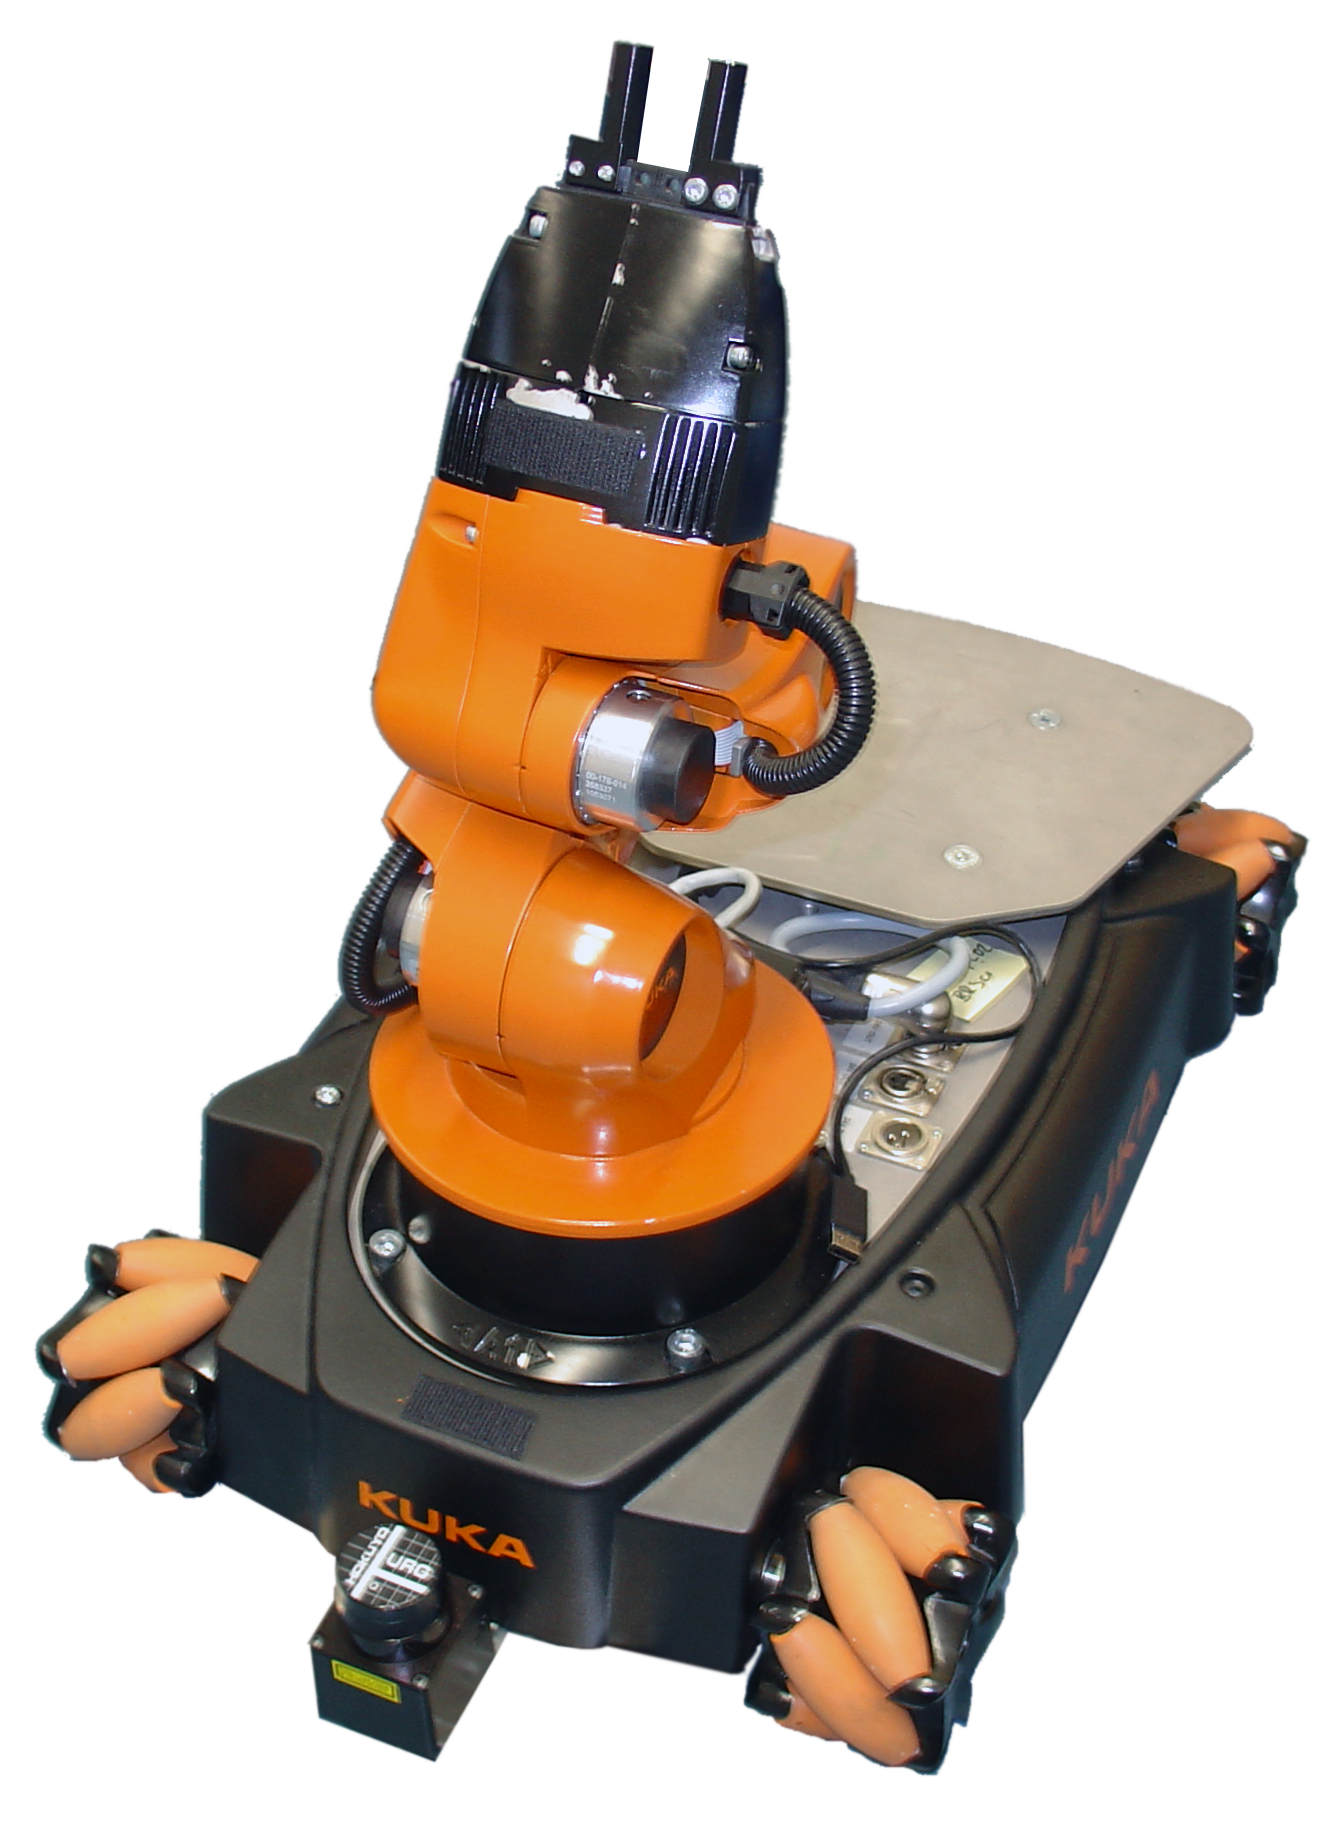
\includegraphics[width=0.60\textwidth]{gfx/youbot.png}
	\textbf{}\\
	\vspace{3 cm} 
	\normalsize
	Author: Frederik Hegger and Jan Paulus\\
    Version: 0.1 (19.11.2012)\\
    
	
\end{center}
\newpage

%%%%%% TABLE OF CONTENTS %%%%%%%%%%
\tableofcontents 
\newpage

%%%%%% MAIN DOCUMENT %%%%%%%%%%%%%%
\section{Ubuntu Distribution}
This installation guide was created while installing the \textit{11.10} (Oneiric) Ubuntu distribution on the internal PC of the youBot. In general, this guide should be also applicable to all other earlier distributions down to \textit{10.04} (Lucid). For future release like \textit{12.04} (Precise) we do not have any experience up to now.



\subsection{User Name(s) and Password(s)}
For the internal and a potential external pc, please use the following information to setup the standard user account
	
\begin{itemize}
	\item User name: b-it-bots
	\item Password: \textit{please ask a staff member for the current password to set}
\end{itemize}

If the Ubuntu installation is succesfully completed, set the root password with same password as used for the previouly mentioned user account:
\begin{lstlisting}
sudo passwd
\end{lstlisting}



\subsection{Add BRSU Mirror Server}
The BRSU mirror servers is located at 
\begin{lstlisting}
http://brics.inf.h-brs.de
\end{lstlisting}
and hosts mirrors for various Ubuntu and ROS release. Please go to the mentioned website and add the information displayed there to the source.list file:
\begin{lstlisting}
sudo nano /etc/apt/source.list
\end{lstlisting}



\subsection{Remove Unused Software}
Some software or tools of the standard Ubuntu installation are not required for a youBot installation. In order to save space, those packages can be removed:
\begin{lstlisting}
sudo apt-get remove deja-dup brasero brasero-cdrkit brasero-common tomboy ubuntuone-control-panel ubuntuone-client gbrainy gnome-mahjongg gnome-sudoku gnomine libreoffice-* shotwell simple-scan empathy gwibber thunderbird transmission-* banshee usb-creator-gtk onboard
\end{lstlisting}



\subsection{Install Additional Software Packages}
Some network tools and other packages are required for latter installation steps:
\begin{lstlisting}
sudo apt-get install openssh-server beep
\end{lstlisting}

\subsection{Cleanup and Update}
Clean up downloaded packages and do an update of the whole system:
\begin{lstlisting}
sudo apt-get clean
sudo apt-get autoclean
sudo apt-get autoremove
sudo apt-get update
sudo apt-get upgrade
sudo apt-get dist-upgrade 
\end{lstlisting}

Remove the default folders from the home directory:
\begin{lstlisting}
rm -rf ~/Documents/ ~/Downloads/ ~/examples.desktop ~/Music/ ~/Pictures/ ~/Public/ ~/Templates/ ~/Videos/
\end{lstlisting}


\subsection{Special Settings}
\begin{itemize}
	\item \textbf{Update manager} $\rightarrow$ disable distribution upgrade in settings of the update manager
	\item \textbf{Power management} $\rightarrow$ don't suspend if inactive	
	\item \textbf{Power management} $\rightarrow$ do nothing if lid is closed
	\item \textbf{Power management} $\rightarrow$ hibernate if power is critical low
	\item \textbf{Screen} $\rightarrow$ dim screen to save power
	\item \textbf{Screen} $\rightarrow$ turn off after 5min
	\item \textbf{Screen} $\rightarrow$ lock: off	
\end{itemize}



\newpage
\section{Network Configuration}
\begin{center}
	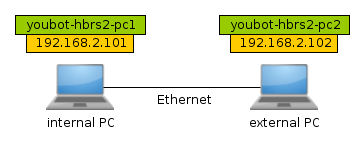
\includegraphics[width=0.60\textwidth]{gfx/network.png}
\end{center}

\subsection{IP Address(es)}

\subsubsection{Ethernet}
In case of an additional laptop beside the internal youBot PC, the network connection needs to be configured. According to the previous paragraph the IP addresses are set as follows:
\begin{lstlisting}
192.168.#.10#
\end{lstlisting}

\begin{itemize}
	\item \textbf{first '\#':} indicates the actual youBot, i.e. for the youot-hbrs2 the IP address space is 192.168.2.10\#
	\item \textbf{second '\#':} indicates the PC ID on a particular youBot, i.e. \textit{youbot-hbrs2-pc1} gets the IP 192.168.2.101 and \textit{youbot-hbrs2-pc2} gets the IP 192.168.2.102.
\end{itemize}

\subsubsection{EtherCAT}
For the EtherCAT connection, a random but valid static IP address is recommended.\\

\textbf{INFO}: do not forget to set the subnet mask to 255.255.255.0

\subsubsection{WLAN}
TDB: connect to youbot-developers, PW, Fritz Stick works plug and play, other stick drivers see wiki, youbot-hbrs2 has not internal wifi, but 1 has


\subsection{Hostname(s)}
If the hostname was not set correct during the installtion, it can be changed by editing the file:
\begin{lstlisting}
sudo nano /etc/hostname
\end{lstlisting}

The hostname of a youbot PC is constructed as follows:
\begin{lstlisting}
youbot-hbrs#-pc#
\end{lstlisting}

\begin{itemize}
	\item \textbf{first '\#':} indicates the actual youBot. At BRSU, there currently exist two youBots, resulting in the names \textit{youbot-hbrs1-pc\#} and \textit{youbot-hbrs2-pc\#}.
	\item \textbf{second '\#':} indicates the PC ID on a particular youBot. The \textit{youbot-hbrs2} has two PCs, the internal and and additional laptop. The internal PC is called \textit{youbot-hbrs2-pc1} and the second laptop \textit{youbot-hbrs2-pc2}.
\end{itemize}

Finally, add the hostname and the related IP address of another youBot PC to the hosts file:
\begin{lstlisting}
sudo nano /etc/hosts
\end{lstlisting}

\subsection{Generate SSH key}
Generate a SSH key pair ...
\begin{lstlisting}
ssh-keygen
\end{lstlisting}

... and copy it to all remote computers on which components need to be launched:
\begin{lstlisting}
cat ~/.ssh/id_rsa.pub | ssh b-it-bots@youbot-hbrs#-pc# 'cat >> ~/.ssh/authorized_keys'
\end{lstlisting}

Now, login once from one PC to the other and vice versa. You should NOT be asked for a password. Otherwise something went wrong in the previous steps.\\

Finally, copy the generated SSH key and add it to the related github account:
\begin{lstlisting}
cat ~/.ssh/id_rsa.pub
\end{lstlisting}

\subsection{NTP Server and Client}
TBD


\newpage
\section{GIT}
Install git version control system and various GUI tools:
\begin{lstlisting}
sudo apt-get install git-core gitg gitk
\end{lstlisting}

Enable auto coloring for git outputs in the terminal:
\begin{lstlisting}
git config --global color.branch auto
git config --global color.diff auto
git config --global color.interactive auto
git config --global color.status auto
\end{lstlisting}



\newpage
\section{youBot Software}

\subsection{RoboCup@Work}
Please follow the instructions on the following webpage to setup the RoboCup@Work software on the youBot:
\begin{lstlisting}
https://github.com/b-it-bots/RoboCupAtWork
\end{lstlisting}

\subsection{Change GIT Remotes}
By default the repositories of the b-it-bots are read-only. In order to push changes from the youBot PCs to a respository, the github user "youbot-hbrs" has a fork for each repository. The remotes can be changed as follows:
\begin{lstlisting}
cd ~/RoboCupAtWork/
git remote rename origin b-it-bots
git remote add origin git@github.com:youbot-hbrs/RoboCupAtWork.git
\end{lstlisting}

\begin{lstlisting}
cd ~/external_software/hbrs-ros-pkg/
git remote rename origin b-it-bots
git remote add origin git@github.com:b-it-bots/hbrs-ros-pkg.git
\end{lstlisting}

\begin{lstlisting}
roscd third-party-software/
git remote rename origin b-it-bots
git remote add origin git@github.com:youbot-hbrs/third-party-software.git
\end{lstlisting}



\subsection{Setup .bashrc}
Please follow the instructions on the following webpage to setup the RoboCup@Work software on the youBot:
\begin{lstlisting}
cd ~/RoboCupAtWork/setup/bashrc
sudo mkdir /etc/youbot
sudo cp youbot-pc#.bashrc /etc/youbot/youbot.bashrc	    
cp user.bashrc ~/.bashrc
\end{lstlisting}

Adapt all aliases, variables like ROBOT, ROBOT\_ENV in the .bashrc file to the needs of the specific youBot.\\

\textbf{INFO}: do not forget to replace the \# with the specific PC ID on which you are working on right now.


\subsection{UDEV Rules}
Copy the predefined udev rules into the rules.d directory:
\begin{lstlisting}
cd ~/RoboCupAtWork/setup/udev_rules
sudo cp 50-youbot-hbrs#-devices.rules /etc/udev/rules.d/
\end{lstlisting}

\textbf{INFO}: do not forget to replace the \# with the specific youBot ID on which you are working on right now.

\subsection{Battery Status Monitor}
The battery status monitor checks the current state of the battery and also the power connection. In case of a drop of the battery level below $ 10\% $, a beep sound will be played on the mainboard speaker. If a roscore is present the voltage information are published as a rostopic. 

\subsubsection{Enable PC-Steaker / Disable Soundcard}
Remove or comment the following line from "/etc/modprobe.d/blacklist.conf"
\begin{lstlisting}
blacklist pcspkr
\end{lstlisting}
    
and add the following line:
\begin{lstlisting}
blacklist snd_hda_intel
\end{lstlisting}
    

\subsubsection{On youbot-hbrs\#-pc1}
\begin{lstlisting}
roscd raw_youbot_battery_monitor
rosmake
sudo cp youbot_battery_monitor.sh ./bin/youbot_battery_monitor /etc/youbot/
\end{lstlisting}


\subsubsection{On youbot-hbrs\#-pc2}
\textbf{WARNING}: TBD
\begin{lstlisting}
roscd raw_laptop_battery_monitor
rosmake
sudo cp youbot_battery_monitor.sh ./bin/youbot_battery_monitor /etc/youbot/
\end{lstlisting}


\subsection{ZeroMQ - RefereeBox Communication}
TBD

\end{document}








